\documentclass[11pt,a4paper]{article}
\usepackage[utf8]{inputenc}
\usepackage{amsmath}
\usepackage{amsfonts}
\usepackage{amssymb}
\usepackage{float}
\usepackage{graphicx}
\usepackage{todonotes}
\usepackage{algorithm}
\usepackage{algpseudocode}

\restylefloat{table}
\title{Project Report: Managing Transfer-Based Datacenter Connections}
\author{Daniel Naro, Maria Gabriela Valdes, Victoria Beleuta}
\begin{document}
\maketitle
\section{Introduction}

For our project we implemented the integer linear programming model described in the paper "Managing Transfer-Based Datacenter Connections" by Adrian Asensio and Luis Velasco. When building large infrastructures, cloud operators are capable of reducing capital expenditures by having a dynamic cloud service that uses under-utilized resources in remote datacenters. Because the amount of data that needs to be transferred is huge, datacenters are interconnected with a flexgrid optical network. As traffic requests come in, resource managers can set up and tear down connections of the necessary bit-rate, for a specified time period needed to accommodate the amount of data to be transferred. For each of these connections, the frequency slot depends on the bandwidth requested.  Elastic connections were suggested due to the fact that not enough resources might be available at the request time. Because of this, managers have to be able to dynamically reschedule the ongoing transferences, i.e. change the frequency slots already allocated, such that there are enough slices to fulfill the new requested connection. These elastic connections are possible through programmable bandwidth-variable transponders that can provide optical signals of different characteristics.\\

For this project we also implemented a Greedy algorithm and a GRASP-like meta-heuristic for the same previously described problem.\\

This project report is structured as follows. We present the integer linear programming (ILP) model implemented in Section 2. Section 3 and 4 defines two meta-heuristic algorithms. The results of our project and a comparison of the results obtained and the performance are detailed in Section 5. Finally, Section 6 concludes the report.

\section{ILP Model}

In order to simplify the spectrum allocation problem, we limited our project to only one new transfer being requested. We have a network topology represented by a graph $G(L,E)$ with a set of locations ($L$) and set of fiber connections ($E$). We are given a subset ($D$) of the data-center's locations. We also know the characteristics of the connections, i.e. a set $S$ of available spectrum slices, and the capacity and number of flows of the optical transponders at each location. The set $R$ contains the ongoing transferences. For each transfer we know the origin ($o_{r}$), destination ($d_{r}$), the remaining amount of data ($v_{r}$) to be transferred, the requested completion time ($c_{r}$), the route ($r_{r}$) and slot currently allocated ($s^{0}_{r}$), the scheduled slot allocation ($s^{1}_{r}$) to be performed at time $t^{1}_{r}$, and the scheduled completion time ($t_{r}$). The details of the new transfer request are given in the tuple $\{o_{r}; d_{r}; v_{r}; c_{r}\}$. The output of our model is the route allocated ($r_{r}$), scheduled completion time ($t_{r}$), bitrate of the connection ($s^{0}_{r}$), the new spectrum allocation ($w^{0}_{r}$), and scheduled reallocation ($w^{1}_{r}$, $t^{1}_{r}$) for each transference that is rescheduled. Our objective is to minimize the number of connections to be rescheduled to make room for the incoming request.\\

% to do: do we need pseudo code for precomputing?
A rescheduling for any transference $r$ needs two spectrum allocations: $s^{0}_{r}$ from time $t_{0}$ to $t^{1}_{r}$ and $s^{1}_{r}$ from time $t^{1}_{r}$ to $t_{r}$, such that the combined area of the two rectangles allows conveying the remaining amount of data $v_{r}$ and $t_{r} \leq  c_{r}$. To decide dimensions, spectrum and time necessary for the ongoing transferences are precomputed. To do this we have written a Java program which precomputes any feasible combination of rectangles $A_{0}$ and $A_{1}$. To obtain these rectangles, we consider discretized time. The sets of rectangles are generated for the ongoing transferences and the requested transfer.\\

\begin{algorithm}[H]
\caption{Generation of rectangles}\label{rectangles_precomputation}
\footnotesize
\begin{algorithmic}[1]
\Procedure{Rectangles\_precomputation}{$transfer, max\_slice$}
	\State $start\_time\_a0 \gets 0$
	\State $compliant\_rectangles\_pair$
	\For{$end\_time\_a0=1 \to transfer.dead\_line$}
		\For{$slice\_start\_a0=0 \to max\_slice$}
			\For{$slice\_end\_a0=slice\_star\_a0 \to max\_slice$}
				\State $tmp\_a0 \gets Rectangle(start\_time\_a0, end\_time\_a0,slice\_start\_a0,slice\_end\_a0)$
				\For{$j=i \to transfer.deadline$}
					\For{$slice\_start_a1=0 \to slice\_start_a0$}
						\For{$slice\_end\_a1=slice\_end\_a0 \to max\_slice$}
							\State $tmp\_a1 \gets Rectangle(start\_time\_a1, end\_time\_a1,slice\_start\_a1,slice\_end\_a1)$
							\If{$transfer.rectanglesCompliant(tmp\_a0, tmp\_a1)$}
								\State $compliant\_rectangles.add(tmp\_a0, tmp\_a1)$
							\EndIf
						\EndFor
					\EndFor		
				\EndFor
			\EndFor
		\EndFor		
	\EndFor
\EndProcedure
\end{algorithmic}
\end{algorithm}

In order to present the ILP model, we define the necessary parameters and variables:

\begin{table}[H]
\small
\begin{tabular}{c l}
$E$ & set of fiber links in the network, index $e$.\\
$S$ &  set of frequency slices, index $s$.\\
$T$ & set of time intervals, index $t$.\\
$R$ & set of ongoing transferences, index $r$.\\
$P$ & set of routes between origin and destination for the new request, index $p$.\\
$A$ & set of candidate areas for the requested trans- ference, index $a$.\\
$A^{0}_{r}$ & set of candidate areas for $r$ between $t_{0}$ and $t^{1}_{r}$ and a spectrum allocation.\\
$A^{1}_{r}$ & set of candidate areas for $r$ between $t_{1}$ and $t_{r}$ and a spectrum allocation.\\
$\omega_{ar}$ & 1 if transference r was assigned to area $a$, 0 otherwise.\\
$\delta_{as}$ & 1 if area a includes slice $s$, 0 otherwise.\\
$\gamma_{at}$ & 1 if area $a$ includes time interval $t$, 0 otherwise.\\ 
$\rho_{pe}$ & 1 if route $p$ uses link $e$, 0 otherwise.\\
$\rho_{re}$ & 1 if transference $r$ uses link $e$, 0 otherwise.\\
$\beta_{raa'}$ & 1 if pair of areas $a \in A_{0}$ and $a' \in A_{1}$ for transference $r$ is feasible.\\
\end{tabular}
\end{table}

Variables:

\begin{table}[H]
\small
\begin{tabular}{c l}
$x_{ap}$ & 1 if the new transference is assigned to area $a$ through route $p$.\\
$y_{r}$ & 1 if transference $r$ is rescheduled, 0 otherwise.\\
$x^{0}_{ar}$ & 1 if transfer $r$ is assigned to area $a \in A_{0}$.\\
$x^{1}_{ar}$ & 1 if transfer $r$ is assigned to area $a \in A_{1}$.\\
\end{tabular}
\end{table}

And the ILP model is as follows:\\\\

$minimize \sum_{r\in R} y_{r} $\\\\

subject to:\\\\

$\sum_{a \in A} \sum_{p \in P}$ $x_{ap} = 1$\\\\
$\sum_{a \in A_{0(r)}}$ $x^{0}_{ar}=1$    $\forall r \in R$\\\\
$\sum_{a \in A_{1(r)}}$ $x^{1}_{ar}=1$    $\forall r \in R$\\\\
$\sum_{a' \in A_{1(r)}}$ $\beta_{raa'}*x^{1}_{a'r} \geq x^{0}_{ar}$     $\forall r \in R,$ $a \in A_{0(r)}$\\\\
$x^{0}_{ar} - \omega_{ar} \leq y_{r}$     $\forall$ $r \in R,$ $a \in A_{0(r)}$\\\\
$\sum_{r \in R} \sum_{a \in A_{0(r)}}$ $\delta_{as} * \gamma_{at} * \rho_{re} * x^{0}_{ar} + \sum_{r \in R} \sum_{a \in A_{1(r)}} \delta_{as} * \gamma_{at} * \rho_{re} * x^{1}_{ar}$\\ 
$+ \sum_{a \in a} \sum_{p \in P} \delta_{as} * \gamma_{at} * \rho_{pe} * x_{ap} \leq 1$    $\forall$ $e \in E,$ $s \in S,$ $t \in {\{t^{0},...,T\}}$\\

The first constraint guarantees that the transfer request is served with route $p$ and rectangle $a$. Then we select the feasible rectangles for the ongoing transferences with the next three constraints. Afterwards, with the fifth constraint we decide whether a transference needs to be reallocated or not and the last constraint guarantees that there are no links used by more than one constraint for each time interval. \\

We have implemented and tested our ILP model with the ILOG CPLEX studio.

\section{Meta-Heuristic Algorithms}

\subsection{Main Algorithm}

To solve the spectrum allocation problem we use the Greedy and GRASP algorithms. Initially we develop a program to precompute all the available paths in the graph between source and destination nodes of the requested transfer using Breadth-first search. Next, we have divided the search for a feasible solution in three main parts: Trivial Case, Half Hard Case and Hard Case, and we analyze in which category the addition of this new transfer falls into.

\subsubsection{Trivial Case}

A trivial case, showed in Figure~\ref{fig:trivial}, happens when adding a new transfer into the network does not require the rescheduling of any of the other scheduled ongoing transfers, because the required number of free slices is already available throughout all of the slices of the assigned path of the new transfer. In Algorithm~\ref{easy_case} you can see the algorithm explained in pseudo-code.\\

\begin{figure}[H]
  \centering
    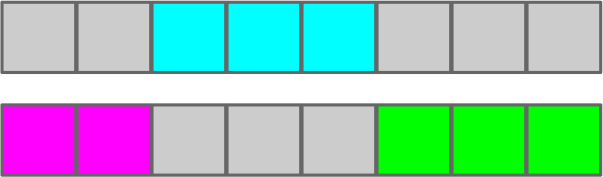
\includegraphics[scale=1]{trivialcase.jpg}
  \caption{Trivial Case}
  \label{fig:trivial}
\end{figure}

\begin{algorithm}[H]
\caption{Easy solution}\label{easy_case}
\begin{algorithmic}[1]
\Procedure{Easy\_solution}{$path, all\_slices, required\_slices$}
	\State $transmission\_collection\gets path.transmission$
	\State $available\_slices\gets all\_slices$
	\ForAll{$transmission \in transmission\_collection$}
      \State $available\_slices \gets available\_slices\setminus transmission.slices$
	\EndFor
	\State $max\_window \gets max\_consecutive\_slices(available\_slices)$
	\State \Return $max\_window \geq required\_slices$
\EndProcedure
\end{algorithmic}
\end{algorithm}

\subsubsection{Half Hard Case}

The half hard case, Figure~\ref{fig:halfhardcase}, implies evaluating the possibility of adding a new transfer into the network. In this scenario only some slices are currently available, but not enough. As a consequence, it is necessary to check on each link, of all of the ongoing transferences, and see if they can be rearranged to increase the time it takes to end the transaction, while still maintaining the completion time constraint, consequently freeing up some slices for the requested transfer. We first check if ``squeezing'' the left transfer to the left we have enough space, if not we try ``squeezing'' the right transfer to the right and check again if we have freed all the slices needed by the new transfer. Algorithm~\ref{half_hard} refers to pseudo-code of this particular case.\\

\begin{figure}[H]
  \centering
    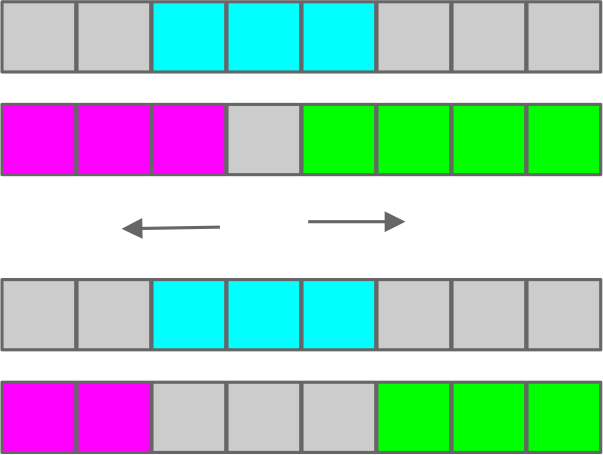
\includegraphics[scale=1]{halfhardcase.jpg}
  \caption{Half Hard Case}
  \label{fig:halfhardcase}
\end{figure}

\begin{algorithm}[H]
\caption{Half hard}\label{half_hard}
\begin{algorithmic}[1]
\Procedure{Half\_hard\_solution}{$path, all\_slices, required\_slices$}
	\State $transmission\_collection\gets path.transmission$
	\State $available\_slices\gets all\_slices$
	\ForAll{$transmission \in transmission\_collection$}
      \State $available\_slices \gets available\_slices\setminus transmission.slices$
	\EndFor
	
	\State $found \gets False$
	\ForAll{$candidate \in consecutive\_slices(available\_slices)$}
		\ForAll{$transmission \in transmission\_collection$}
			\State $transmission.free\_around\_candidate(candidate)$
		\EndFor
		\State $candidate.update()$
		\If $candidate.size \geq required\_slices$
			\State $found \gets True$
			\State $Break$
		\EndIf
	\EndFor
	\State \Return $found$
\EndProcedure
\end{algorithmic}
\end{algorithm}

\subsubsection{Hard Case}

When we do not have any free slices available in any link throughout the selected path, we have a hard case, Figure~\ref{fig:hardcase}. In this particular case, we have to perform the same ``squeezing'' procedure specified in the previous case, but first we have to check each intersection point between two ongoing transferences to select a starting point where we can insert the new transfer that needs to be scheduled. Once we have found an intersection which we can expand enough to make room for the requested transfer, we have to check on the other links if the expansion is also possible there. Once we have found an intersection which we can expand enough to make room for the requested transfer, we have to check on the other links if the expansion is also possible there. More details about this case can be seen in Algorithm~\ref{hard} pseudo-code.\\

\begin{figure}[H]
  \centering
    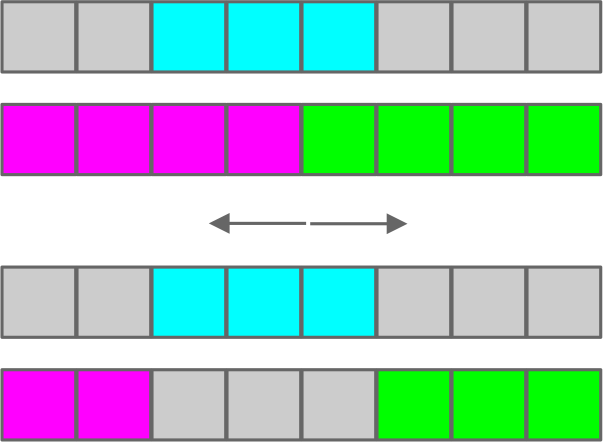
\includegraphics[scale=1]{hardcase.jpg}
  \caption{Hard Case}
  \label{fig:hardcase}
\end{figure}

\begin{algorithm}[H]
\caption{Hard}\label{hard}
\begin{algorithmic}[1]
\Procedure{hard\_solution}{$path, all\_slices, required\_slices$}
	\State $transmission\_collection\gets path.transmission$
	\State $available\_slices\gets all\_slices$
	\State $candidates\_collection\gets new Set()$
	\ForAll{$transmission \in transmission\_collection$}
      \State $candidates\_collection.insert(transmission.first\_slice)$
      \State $candidates\_collection.insert(transmission.last\_slice)$
	\EndFor
	
	\State $found \gets False$
	\ForAll{$candidate \in candidates\_collection$}
		\ForAll{$transmission \in transmission\_collection$}
			\State $transmission.free\_around\_candidate(candidate)$
		\EndFor
		\State $window\_size=getSizeWindowCreated()$
		\If $window\_size \geq required\_slices$
			\State $found \gets True$
			\State $Break$
		\EndIf
	\EndFor
	\State \Return $found$
\EndProcedure
\end{algorithmic}
\end{algorithm}

\subsection{Greedy}
For our first meta-heuristic, we used the Greedy algorithm that iterates through all the precomputed paths, going through all the previously defined cases to find a feasible solution. If a solution is found for a given path, the loop termites and the rest of the paths are not checked.
 
\subsection{GRASP-like Method} 

\subsubsection{Construction Phase}

For the second meta-heuristic we implemented a GRASP-like algorithm. The precomputed paths mentioned earlier are sorted by length or number of hops to create our set $C$ of candidates. Using an alpha parameter of 0.3 we select only the best subset of smallest found paths, this is, the RCL set. For each of the three types of solutions we iterate ten times over the paths in the RCL: we select one at random and try to solve it according to the current section. We have a book-keep in each of the three sections to maintain a list of visited paths such that we do not select twice the same option. The general algorithm is described as pseudo-code in Algoritm~\ref{grasp}.\\

The shorter the path, the more likely it is that we will need less reschedulings. With repeatedly random selection we have seen improvement in our optimization: all those cases where the first path returned by the BFS was not the best one, are now improved. The problem is that we need more time to sort the data, retry repeatedly, etc.

\begin{algorithm}[H]
\caption{GRASP-like}\label{grasp}
\begin{algorithmic}[1]
\Procedure{GRASP\_like}{$graph, requested\_transfer, ongoing\_transfers$}
	\State $pathes \gets graph.bfs(requested\_transfer)$
	\State $pathes.apply(ongoing\_transfers)$
	\State $sort(pathes)$

	\State $RCL \gets pathes.select(pathes.min, pathes.min+RCL.\alpha*(pathes.max-pathes.min)$
	\State $minReschedules \gets \infty$
	\State $bestReschedule \gets null$

	\For{$i=0 \to 10$}
		\State $RCL.discard(visited\_trivial)$
		\State $path \gets selectRandom(RCL)$
		\State $currentReschedule \gets Easy\_solution(path)$
		 \If{$currentReschedule.reschedules \leq minReschedules$}
			\State $minReschedules \gets currentReschedule.reschedules$
			\State $bestReschedule \gets currentReschedule$
		\EndIf
		\State $visited\_trivial.add(path)$
	\EndFor

	\If{$minReschedules\geq 0$}
		\For{$i=0 \to 10$}
			\State $RCL.discard(visited\_HalfHard)$
			\State $path \gets selectRandom(RCL)$
			\State $currentReschedule \gets HalfHard\_solution(path)$
			 \If{$currentReschedule.reschedules \leq minReschedules$}
				\State $minReschedules \gets currentReschedule.reschedules$
				\State $bestReschedule \gets currentReschedule$
			\EndIf
			\State $visited\_HalfHard.add(path)$
		\EndFor
		\For{$i=0 \to 10$}
			\State $RCL.discard(visited\_Hard)$
			\State $path \gets selectRandom(RCL)$
			\State $currentReschedule \gets Hard\_solution(path)$
			 \If{$currentReschedule.reschedules \leq minReschedules$}
				\State $minReschedules \gets currentReschedule.reschedules$
				\State $bestReschedule \gets currentReschedule$
			\EndIf
			\State $visited\_Hard.add(path)$
		\EndFor

		\State $localSearch(bestReschedule)$
	\EndIf
\EndProcedure
\end{algorithmic}
\end{algorithm}

\subsubsection{Local Search}

The local search of our GRASP algorithm consists of using as an input all the free slices obtained after deciding the reschedulings to be done. If we have more slices available than the ones required for the requested transfer, we check if we can safely undo some of the reschedule decided in the construction phase. We then choose the undoing which gives us the minimal of total reschedulings needed.\\

The decision process is straightforward. We iterate over the set of available slices, and select a window of consecutive slices. This window has to be as long as the minimal number of slices needed. We then test if some of reschedulings consisted in liberating slices which are not in our window. All those reschedulings can then be safely undone. Of course we select as the best answer the window which enables us to undo as many reschedulings as possible. Below the pseudo-code of this search in Algoritm~\ref{local_search}.\\ 

\begin{algorithm}[H]
\caption{Local Search}\label{local_search}
\begin{algorithmic}[1]
\Procedure{local\_search}{$window\_available, required\_slices, reschedules\_done$}
	\State $MaxUndoesPossible \gets -1$
	\State $BestUndoCollection \gets null$
	\For{$i=0 \to window\_available-required\_slices$}
		\State $UndoCollection \gets new Set()$
		\State $undo\_candidate \gets [window\_available[0]..window\_available[i-1]] \cup [window\_available[i+required\_slices]..window\_available[end]]$
		\State $undoes\_possible\gets 0$
		\ForAll($transmission \in reschedules\_possible$)
			\If{$transmission.undo\_possible(undo\_candidate)$}
				\State $undoes\_possible++$
				\State $UndoCollection.add(transmission.validate\_undo())$
			\EndIf
		\EndFor
		\If{$undoes\_possible \geq MaxUndoesPossible$}
			\State $MaxUndoesPossible \gets undoes\_possible$
			\State $MaxUndoesPossible \gets UndoCollection.add		(transmission.validate\_undo())$
		\EndIf
	\EndFor
	\State \Return $reschedules\_done.size - MaxUndoesPossible$
\EndProcedure
\end{algorithmic}
\end{algorithm}

\section{Results}
As we have said, the different solutions need some previous work before starting the resolution: in the case of the ILP it is the precomputation of the rectangles and the paths, in the case of the metaheuristics it is just the BFS. We have decided to include the time needed for the precomputation in each of the results we present in this section since in any case it is an important step in the resolution of the transfer schedule.

\subsection{Test 1: inputTestHardAndHalfHard.txt}

\textit{Requested Transfer}: from node \textbf{a} to node \textbf{e}.\\

\begin{figure}[H]
  \centering
    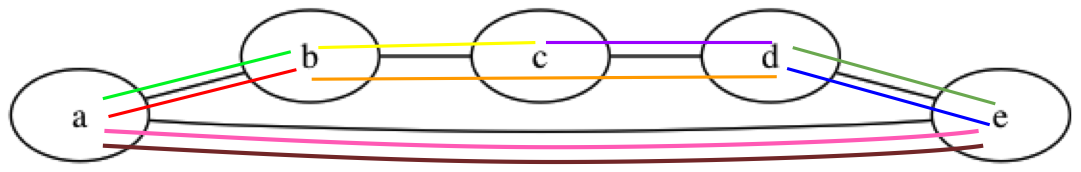
\includegraphics[scale=0.7]{inputTestHardAndHalfHard.png}
  \caption{Test 1}
  \label{fig:test1}
\end{figure}

\begin{tabular}{| l | l | l | l |}
\hline
 & CPLEX & Greedy & GRASP \\ \hline
Result & 1 & 1 & 1 \\ \hline
Total Time & 185.8 & 60 & 110 \\ \hline
\end{tabular}\\\\

In this example we combine two paths, one with a half-hard solution, the other with a hard solution. The optimal solution is found by rescheduling the half-hard path. The main question is if the Greedy version will take advantage of the fact it will not even check the hard path. Effectively, the time needed by Greedy is clearly the lowest in this scenario.

\subsection{Test 2: inputTestHardAndTrivial.txt}

\textit{Requested Transfer}: from node \textbf{a} to node \textbf{e}.\\

\begin{figure}[H]
  \centering
    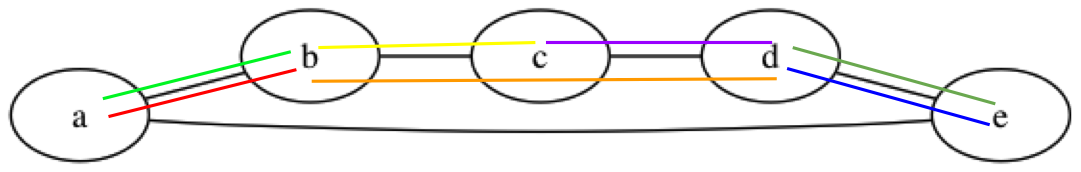
\includegraphics[scale=0.7]{inputTestHardAndTrivial.png}
  \caption{Test 2}
  \label{fig:test2}
\end{figure}

\begin{tabular}{| l | l | l | l |}
\hline
 & CPLEX & Greedy & GRASP \\ \hline
Result & 0 & 0 & 0 \\ \hline
Total Time & 111.7 & 71 & 88 \\ \hline
\end{tabular}\\\\

In this test the obvious solution is to choose the path without any transmissions: all implementations choose this solution. Greedy and GRASP detect this solution right at the beginning, shortening the execution.

\subsection{Test 3: inputTestCombinationIntersectionsSegments.txt}

\textit{Requested Transfer}: from node \textbf{a} to node \textbf{e}.\\

\begin{figure}[H]
  \centering
    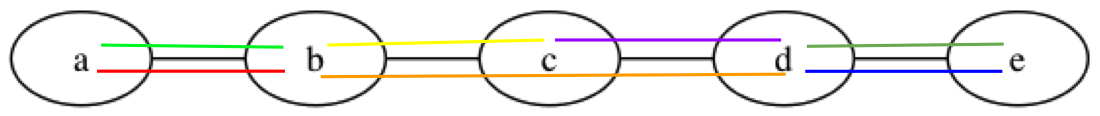
\includegraphics[scale=0.7]{inputTestCombinationIntersectionsSegments.png}
  \caption{Test 3}
  \label{fig:test3}
\end{figure}

\begin{tabular}{| l | l | l | l |}
\hline
 & CPLEX & Greedy & GRASP \\ \hline
Result & 5 & 5 & 5 \\ \hline
Total Time & 291 & 58 & 98 \\ \hline
\end{tabular}\\\\

In this test we have just one path, with many transmissions, defined in such a way that they form a hard solution. We compare how long will the meta-heuristics take to deal with this more complex problem, with the time needed by CPLEX. The result is a clear win for the meta-heuristics: even without taking into account the pre-computation needed before executing CPLEX, the meta-heuristics are faster. It is clear that the Java-code can deal better with the greater number of transmissions.

\subsection{Test 4: inputTestHalfHard.txt}

\textit{Requested Transfer}: from node \textbf{a} to node \textbf{c}.\\

\begin{figure}[H]
  \centering
    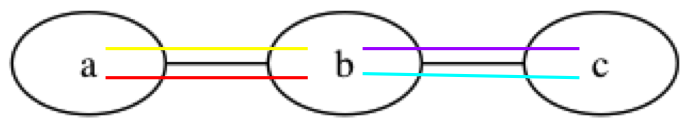
\includegraphics[scale=0.7]{inputTestHalfHard.png}
  \caption{Test 4}
  \label{fig:test4}
\end{figure}

\begin{tabular}{| l | l | l | l |}
\hline
 & CPLEX & Greedy & GRASP \\ \hline
Result & 1 & 2 & 2 \\ \hline
Total Time & 151.4 & 64 & 82 \\ \hline
\end{tabular}\\\\

Let us remember how the rectangles are precomputed for the ILP: we consider all rectangles combinations starting from the slice 0 to the maximal slice. This mean that in some cases CPLEX could prefer to change entirely the set of frequencies used by one of the transmission. For example if one transfer used the slices 3,4,5, the solution of the ILP might decide to assign the slices 1,2.  On the other hand, the meta-heuristic will reschedule the slices in such a way that either the lowest slice or the highest slice will be conserved. This means that CPLEX can return results that the meta-heuristic could never reach.\\

In this example, CPLEX does one of this total frequency shift. This is why the result obtained in the ILP is unreachable by the other two methods.

\subsection{Test 5: inputSeeDifferencesGreedyCplex.txt}

\textit{Requested Transfer}: from node \textbf{a} to node \textbf{e}.\\

\begin{figure}[H]
  \centering
    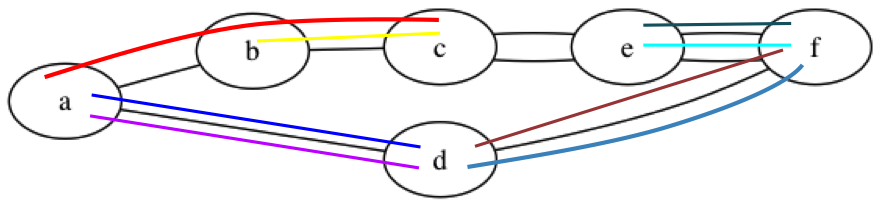
\includegraphics[scale=0.7]{inputSeeDifferencesGreedyCplex.png}
  \caption{Test 5}
  \label{fig:test5}
\end{figure}

\begin{tabular}{| l | l | l | l |}
\hline
 & CPLEX & Greedy & GRASP \\ \hline
Result & 1 & 3 & 2 \\ \hline
Total Time & 135 & 61 & 97 \\ \hline
\end{tabular}\\\\

In this example, we have two paths available. One provide a so called half-hard solution, the other a hard solution. As always CPLEX finds the optimal solution: it is possible to find it by rescheduling over the hard path. However CPLEX changes all the frequencies of one transmission to reach this result. The Greedy implementation returns the solution found with the half-hard implementation, but the GRASP-like keeps running and find a better solution over the hard path.

\subsection{Test Greedy vs. Grasp}

\begin{tabular}{| l | l | l | l |}
\hline
 & CPLEX & Greedy & GRASP \\ \hline
Result & 1 & 2 & 1 \\ \hline
Total Time & 205.6 & 61 & 93 \\ \hline
\end{tabular}\\\\

In this example we provide different seven paths, all of which are hard. Each of the path requires two reschedulings to make space for the new transfer, all except one where it is possible to do it with just one reschedule. CPLEX finds this solution but needs a long time. The Greedy solution is fast, but stops as soon as it has a solution, which in this case is not the optimal one. Our GRASP-like implementation, keeps iterating and ends up finding this solution: it takes longer than the Greedy solution, but in this case the solution is as good as the one from CPLEX.

\subsection{Test 6: inputTestHard.txt}

\textit{Requested Transfer}: from node \textbf{a} to node \textbf{c}.\\
\textit{Number of hard paths}: 1.\\

\begin{figure}[H]
  \centering
    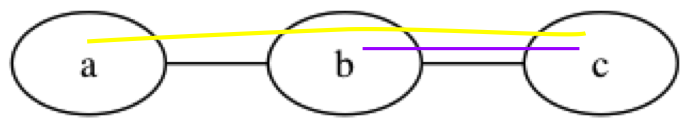
\includegraphics[scale=0.7]{inputTestHard.png}
  \caption{Test 6}
  \label{fig:test6}
\end{figure}

\begin{tabular}{| l | l | l | l |}
\hline
 & CPLEX & Greedy & GRASP \\ \hline
Total Time & 87.2 & 42 & 76 \\ \hline
\end{tabular}

\subsection{Test 7: inputTest2Hard.txt}

\textit{Requested Transfer}: from node \textbf{a} to node \textbf{c}.\\
\textit{Number of hard paths}: 2.\\

\begin{figure}[H]
  \centering
    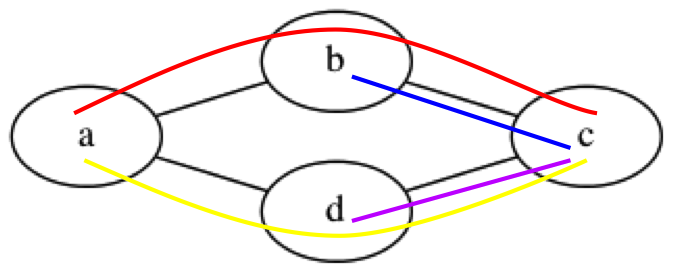
\includegraphics[scale=0.7]{inputTest2Hard.png}
  \caption{Test 7}
  \label{fig:test7}
\end{figure}

\begin{tabular}{| l | l | l | l |}
\hline
 & CPLEX & Greedy & GRASP \\ \hline
Total Time & 107 & 56 & 104 \\ \hline
\end{tabular}

\subsection{Test 8: inputTest3Hard.txt}

\textit{Requested Transfer}: from node \textbf{a} to node \textbf{c}.\\
\textit{Number of hard paths}: 3.\\

\begin{figure}[H]
  \centering
    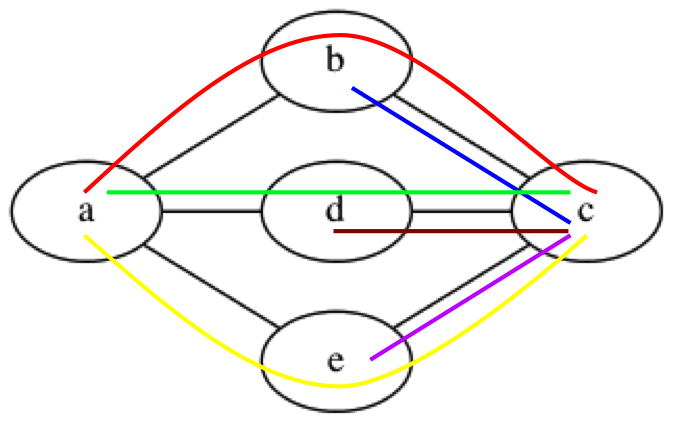
\includegraphics[scale=0.7]{inputTest3Hard.png}
  \caption{Test 8}
  \label{fig:test8}
\end{figure}

\begin{tabular}{| l | l | l | l |}
\hline
 & CPLEX & Greedy & GRASP \\ \hline
Total Time & 168.9 & 81 & 107 \\ \hline
\end{tabular}

\subsection{Test 9: inputTest5Hard.txt}

\textit{Requested Transfer}: from node \textbf{a} to node \textbf{c}.\\
\textit{Number of hard paths}: 5.\\

\begin{figure}[H]
  \centering
    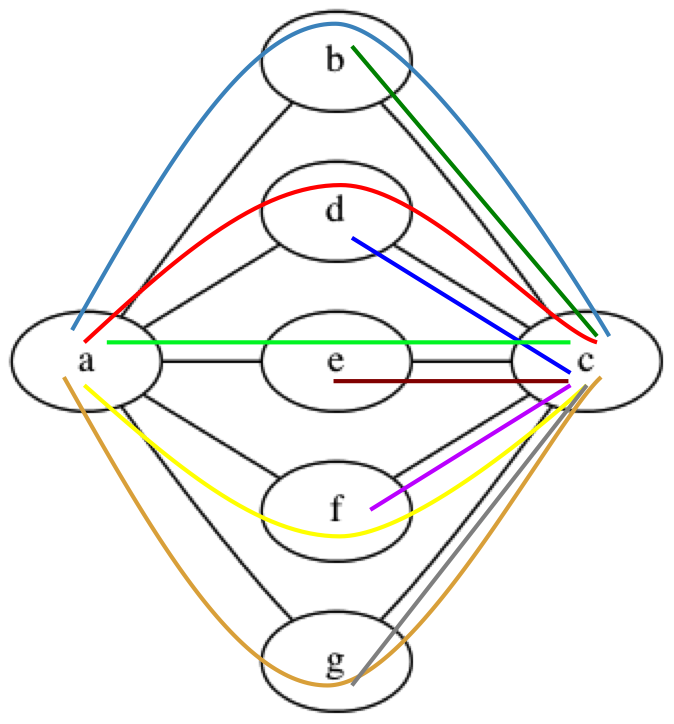
\includegraphics[scale=0.6]{inputTest5Hard.png}
  \caption{Test 9}
  \label{fig:test9}
\end{figure}

\begin{tabular}{| l | l | l | l |}
\hline
 & CPLEX & Greedy & GRASP \\ \hline
Total Time & 177.7 & 71 & 125 \\ \hline
\end{tabular}

\subsection{Test 10: inputTest7Hard.txt}

\textit{Requested Transfer}: from node \textbf{a} to node \textbf{c}.\\
\textit{Number of hard paths}: 7.\\

\begin{figure}[H]
  \centering
    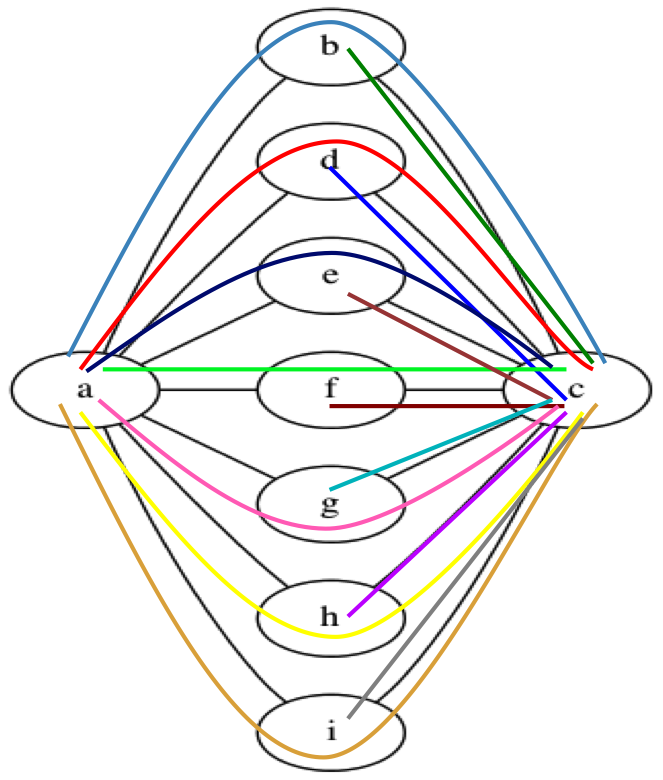
\includegraphics[scale=0.7]{inputTest7Hard.png}
  \caption{Test 10}
  \label{fig:test10}
\end{figure}

\begin{tabular}{| l | l | l | l |}
\hline
 & CPLEX & Greedy & GRASP \\ \hline
Total Time & 253.6 & 79 & 125 \\ \hline
\end{tabular}

\subsection{Performance Comparison: CPLEX vs. Greedy vs. GRASP}

\begin{figure}[H]
    \hspace*{-3cm}
	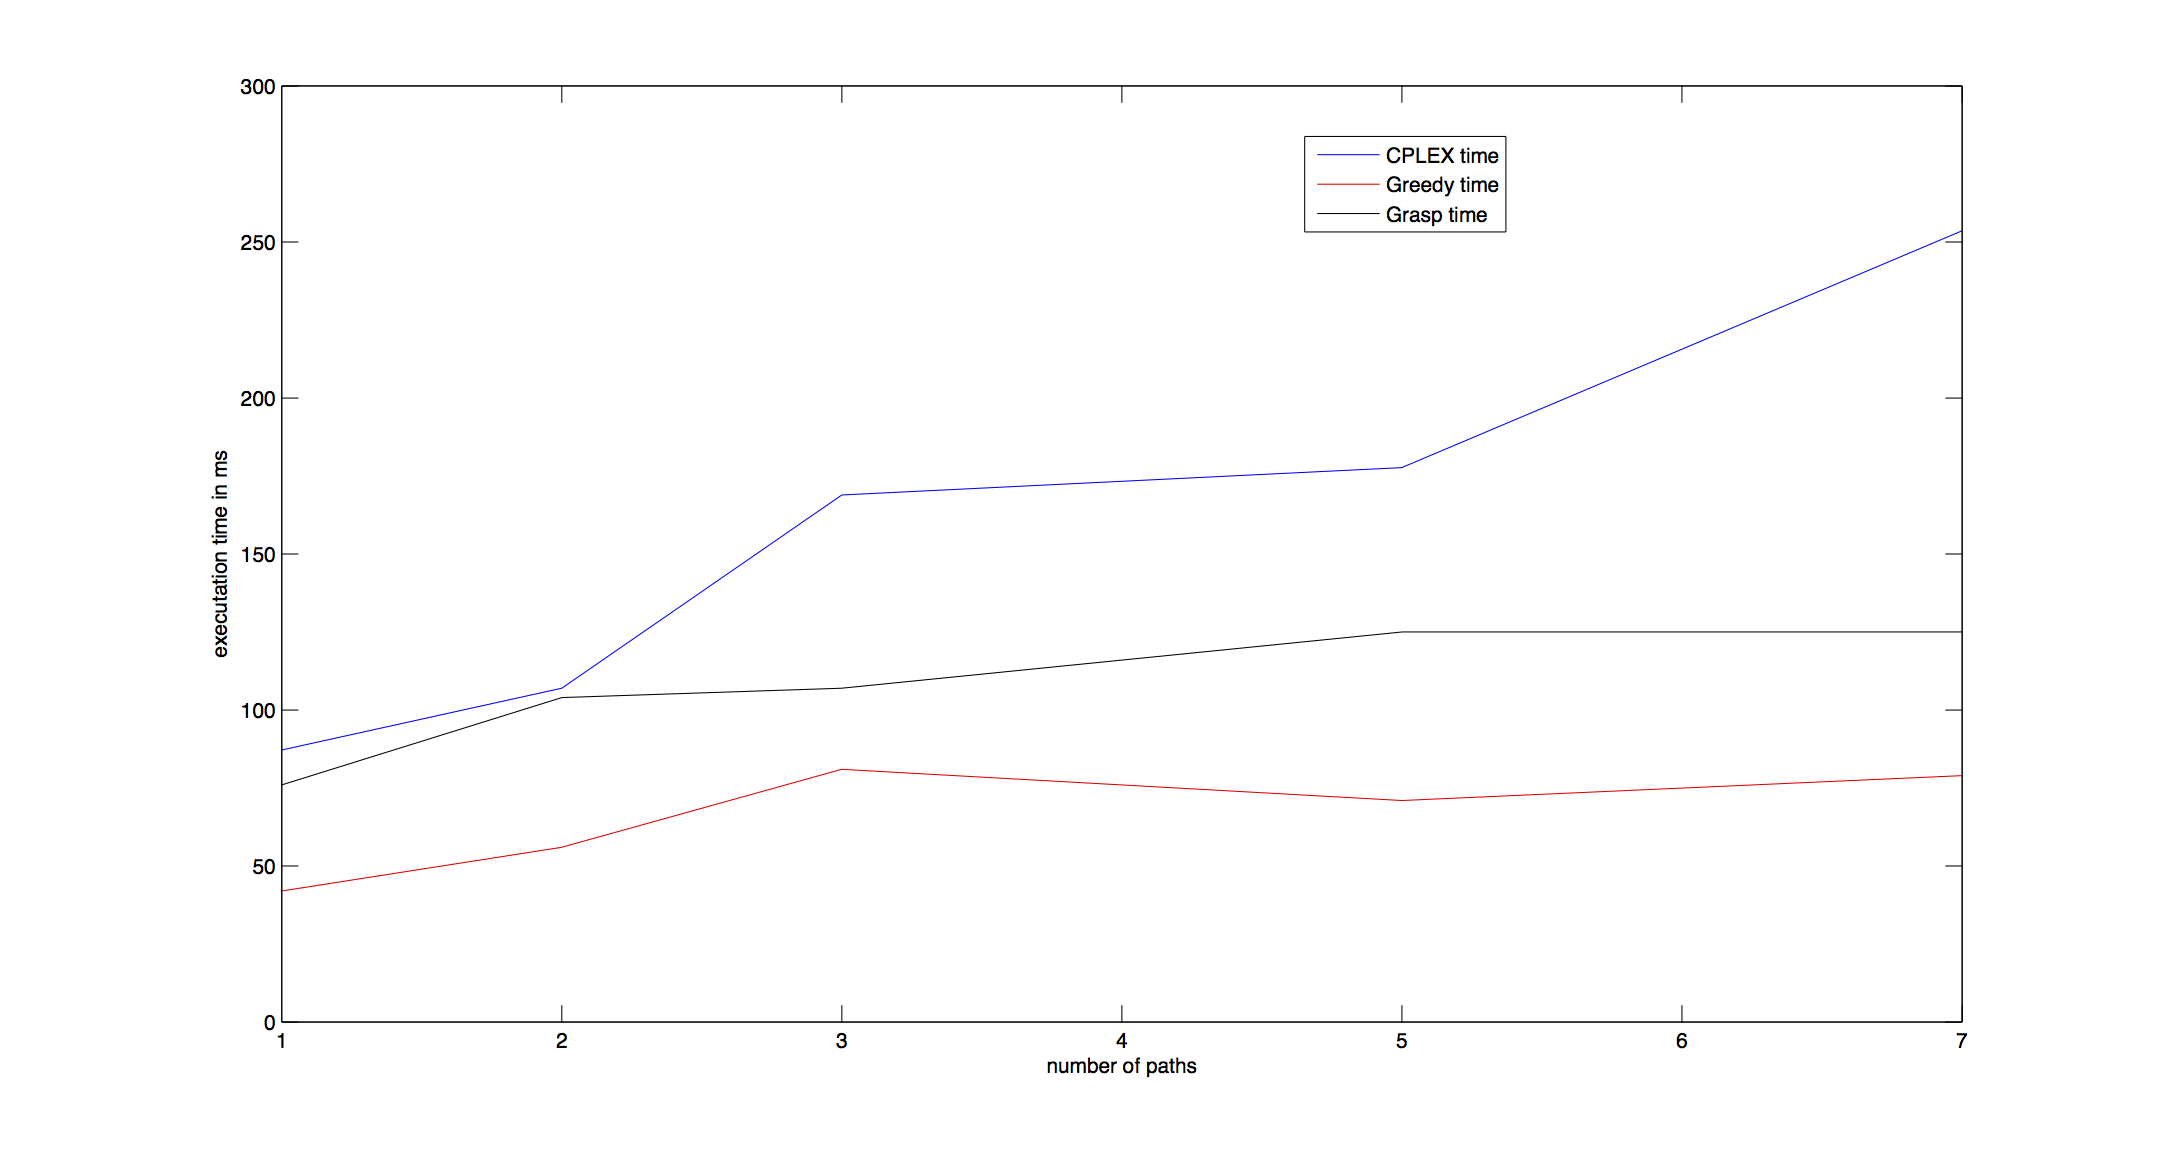
\includegraphics[scale=0.5]{executionTimeGraph.png}
  \caption{CPLEX vs. Greedy vs. GRASP}
  \label{fig:performance}
\end{figure}

The results seen on Figure~\ref{fig:performance} make reference to the previous tests referred in Figures~\ref{fig:test6}, \ref{fig:test7}, \ref{fig:test8}, \ref{fig:test9}, and \ref{fig:test10}. This results clearly show that Greedy finds a feasible solution with better performance than CPLEX and GRASP alternatives. As expected, CPLEX solution tends to increase exponentially with the number of hard paths added to the graph. GRASP algorithm is not affected that badly by the increase of hard paths in the graph, but we can see that for this tipy of tests, randomness doesn't contribute to have a better performance.

\section{Conclusion}
\end{document}
